\section{Implementation}
\label{implementation}

The first CTFEF was created for the C-=-1 language, using generic parser generator and Backend.
The most important aspect of implementing a CTFEF compiler is the design of the data structures, described in chapter \ref{data_structures}, that will be used by the interpreter.

In order to exploit CTFEF approach in design of a compiler, the language should contain a set of data structures to describe user code, i.e. a Semantic Model.
It will allow the programmer to interact and mainpulate the structure of the program at compile-time.
The Semantic model designed and implemented for C-=-1 is described in chapter \ref{semantic_model}.

The final part of a CTFEF compiler is the Backend Interface.
It is a program, written in the target language, and ran at compile-time that translates the semantic model into the Backends' assembly language.
Backend Interface implemented for C-=-1 is relativley small and is described in chapter \ref{implementation/Backend-interface}.

\begin{figure*}
	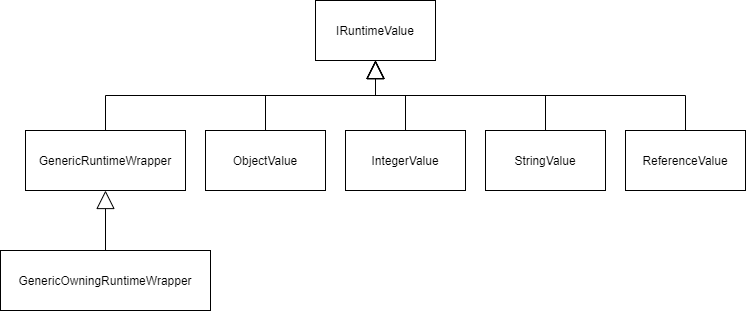
\includegraphics[width=16cm]{pictures/interpreter_data_structures_uml.png}
	\caption{Class diagram of C-=-1 interpreter data structures}
	\label{fig:interpreter_data_structures}
\end{figure*}

\subsection{Interpreter data structures}
\label{data_structures}
Data structures of the C-=-1 Interpreter have been designed having the ease of development and debugging in mind.
They are thus not particularly efficent.

Figure \ref{fig:interpreter_data_structures} contains a class diagram of most of the types used to represent values within C-=-1.
All of them derive from \lstinline{IRuntimeValue} and are managed via C++ smart pointers.
The interface of the base class allows the value to be converted to a human-readable format, serialization, deserialization and copying.

The most primitive types within the hierarchy are \lstinline{StringValue} and \lstinline{IntegerValue}.
They are simple wrappers for strings and integers, present in the host language.
Floating point numbers were not implemented as they were not necessary for implementation of a basic compiler.

User-defined types are represented using \lstinline{ObjectValue}.
The contents of an object is kept as a \lstinline{string} - \lstinline{IRuntimeValue} dictionary, with field names as keys and \lstinline{uniqe_ptr<IRuntimeValue>} as values.
C-=-1 object is therefore spread out in memory, even if the fields are directly contained within the class, without any indirection.


There are several types of reference within the C-=-1 interpreter.
The most basic pointer type is a reference to C-=-1 value.
It was realised as a pointer to the owning pointer of the value.
The reasoning behind this decision was to allow assigning to the referenced value.

\subsection{Program semantic model}
\label{semantic_model}

A major motivation for creating CTFEF was the ability to support languages with compile-time metaprogramming.
This includes reflection and modification of the code being compiled.
User program has to be represented as a complete and modifiable object, using the interpreters' data structures.

C-=-1 language model divides the user program into assemblies.
They represent an individual program package: a library or an executable file.
The compiler is invoked to compile an assembly, together with its dependencies.
Assembly is the root object of C-=-1 program model, it stores a list of assemblies it depends on and the root namespace of the package it represents.
The remainder of user code is organised into namespaces, types, functions and fields.
These parts of the model are represented by native classes of the host language and form the basis for the rest of the model.

The most complex part of the model is the representation of the function body.
Like in most programming languages, a C-=-1 function can contain a variety of instruction types.
That includes complex statements and blocks of statements that can be arbitrarly nested.
Each instruction may also contain expressions of any complexity.

To deal with this complexity, C-=-1 semantic model for functions is build around two interfaces: \lstinline{IInstruction} and \lstinline{IExpression} and their concrete implementations.
Every category of instruction or expression is represented by its own type.
The user may then analyze the structure of the program, using a dynamic type conversion mechanism similar to C++ \lstinline{dynamic_cast} \cite{ISO:cpp98}.

All elements of the semantic model, have a \lstinline{sourcePointers}.
It is a simple structure, that contains the filename and the line number of the expression or instruction.
This information can be passed to compiler intrinsic functions, such as \lstinline{raiseError}, to generate error messages for the user.
Listing \ref{lst:noDiscardCm1} contains an example use of this functionality.
The \lstinline{pointerToSource} makes the messages generated by the compiler easier to understand for the programmer.

Component responsible for creating the semantic model are a major part of the compiler.
There are two operations that this module performs: building the definition of the types used to describe a program, and creating an instance of the model, given semantic information.
C-=-1 compiler has a hard-coded definition of its base library.
It contains definitions of primitive types and types used to build the semantic model of a program.
The description of this library must be built manually, as it is very closley integrated with the compiler.

\subsection{Backend interface}
\label{implementation/Backend-interface}

The C-=-1 Backend interface uses LLVM \cite{llvmir} code generation API that has been exposed by the compiler.
The functionality which has been made available to C-=-1 represents a minimal subset of LLVM, that is sufficient to implement a basic compiler.

Besides translating user code, the Backend Interface must also generate the assembly for certain intrinsic operations.
Functions such as integer arithmetic operators, array indexers or memory allocators are concepts too low-level to be expressed in C-=-1.
They are therefore expressed as functions, without bodies, which are then replaced by appropriate intrinsic operations.

Listing \ref{impl:theoretical_llvmir} contains a simple function written in C-=-1 (line 2), its ideal LLVMIR (line 5) and LLVMIR generated by C-=-1 compiler (line 21).
The current implementation generates a function for each operator, regardless of whether it was defined by the programmer or is a primitive operation.
They are merely a wrapper around the actual LLVM intrinsic, meant to simplify implementation of the Backend Interface.
Future versions, with additional effort, may generate the ideal LLVMIR from line 21 of Listing \ref{impl:theoretical_llvmir}.

Certain other intrinsic operations are defined using external dependencies.
C-=-1 memory management library, in the runtime context, uses a simple interface capable of allocating and deleting a continuous buffer.
It consists of two functions: \lstinline{unsafe_new} and \lstinline{delete}.
In the standard library, they are explicitly mapped to \lstinline{malloc} and \lstinline{free} functions from the C runtime.

Backend interface must also allow the programmer to influence how the executable code is generated.
There are many practical reasons for this capability.
Specifying the name of a function, in order to link it to an external symbol is one of them.
For example, C-=-1 standard library uses \lstinline{malloc} and \lstinline{free} to manage memory.
These symbols are imported as \lstinline{unsafe_new} and \lstinline{delete} in excerpt in Listing \ref{lst:new}.
This is accomplished using the \lstinline{mapToExternalSymbol} attribute and specifying the symbol name as a parameter, as was done in lines zero and three.

\begin{minipage}{\linewidth}
	\begin{lstlisting}[
	tabsize=2,
	numbers=left,
	stepnumber=1,
	caption={Representation of average function in C-=-1 and LLVM IR},
	label={impl:theoretical_llvmir}
	]
// C-=-1 function in source code
fn average(a: usize, b: usize, c: usize) -> usize {
	return (a + b + c) / 3;
}
// Ideal representation in LLVMIR
define i32 @average(i32 %0, i32 %1, i32 %2){
  %4 = add i32 %1, %0
  %5 = add i32 %4, %2
  %6 = sdiv i32 %5, 3
  ret i32 %6
}
// Generated LLVM IR
define i32 @__operator___plus____usize__usize(i32 %0, i32 %1){
	%3 = add i32 %1, %2
	ret i32 %3
}
define i32 @__operator___div____usize__usize(i32 %0, i32 %1){
	%3 = sdiv i32 %1, %2
	ret i32 %3
}
define i32 @average(i32 %0, i32 %1, i32 %2){
	%4 = call __operator___plus____usize__usize(i32 %1, i32 %0)
	%5 = call __operator___plus____usize__usize(i32 %4, i32 %2)
	%6 = call __operator___div____usize__usize (i32 %5, i32 3)
	ret i32 %6
}
\end{lstlisting}
\end{minipage}


One of the possible ways of achieving this, is to declare an interface for an attribute generating a functions symbol name.
Listing \ref{lst:selected_Backend_interface} contains relevant code of a Backend Interface that uses such an attribute, to override mark external symbols.
Interface \lstinline{ISymbolNameOverride} contains only one method: \lstinline{createSymbolName} that returns the name of the symbol in the generated assembly.

Functions \lstinline{buildFunction} and \lstinline{getFunctionName}, from Listing \ref{lst:selected_Backend_interface}, are parts of Backend Interface.
They are invoked in order to convert a C-=-1 \lstinline{functionDescriptor} to a LLVMIR function.
They were included in the Listing, because they are the only parts of the Backend Intreface that need to interact with \lstinline{ISymbolNameOverride} attributes.
Both of these procedures, check whether an attribute implementing this interface is attached to the function they are currently processing.
This happens on lines three and nineteen of Listing \ref{lst:selected_Backend_interface}.
If that attribute is present, code of that function is ignored, and it is treated as an external symbol: condition on line twenty ommits execution of \lstinline{build_block} function on line twenty-three.
Procedure \lstinline{getFunctionName} contains a similar condition on line three, that decides how the name should be generated.
If an \lstinline{ISymbolNameOverride} attribute is present, it will be created by \lstinline{createSymbolName} method of the attribute attached to the function.
Otherwise, the \lstinline{mangleName} function will create name of function's symbol based on its parameters and return type.

\begin{minipage}{\linewidth}

	\begin{lstlisting}[
	  numbers=left,
	  firstnumber=0,
	  caption={C-=-1 memory allocation functions from standard library},
	  aboveskip=0pt,
	  label={lst:new}
	  ]
[mapToExternalSymbol("malloc", "")]
private fn unsafe_new(size: usize) -> char* {}

[mapToExternalSymbol("free", "")]
internal fn delete<typename T>(val: T*) {}

  \end{lstlisting}
\end{minipage}


\begin{minipage}{\linewidth}

	\begin{lstlisting}[
	  numbers=left,
	  firstnumber=0,
	  caption={Part of a Backend Interface, using \lstinline{ISymbolNameOverride} interface},
	  aboveskip=0pt,
	  label={lst:selected_Backend_interface}
	  ]

  private fn getFunctionName(f: functionDescriptor) -> string {
	let attribute = f.get_attribute<ISymbolNameOverride>();
	if(attribute != null<ISymbolNameOverride>())
	  return attribute.createSymbolName();
	return mangleName(f);
  }

  private fn buildFunction(
	f: functionDescriptor,
	llvmF: llvmFunction,
	registry: packageRegistry*,
	mod: llvmModule)
  {
	let variables = dictionary<variableDescriptor, llvmValue>();
	let params = f.parameters();
	for(i in enumerate(0, params.length()))
	  variables.push(params[i], llvmF.getParameter(i));
	let builder = llvmF.getBuilder();
	let attribute = f.get_attribute<ISymbolNameOverride>();
	if(attribute == null<ISymbolNameOverride>())
	{
	  let code = f.code();
	  build_block(&code, &builder, &variables, registry);
	}
  }

  \end{lstlisting}
\end{minipage}


